\documentclass{standalone}
\usepackage{tikz}
\usepackage{xcolor}

\usetikzlibrary{decorations.pathmorphing}
\usetikzlibrary{shapes}
\usetikzlibrary{shapes.geometric}

\begin{document}
	
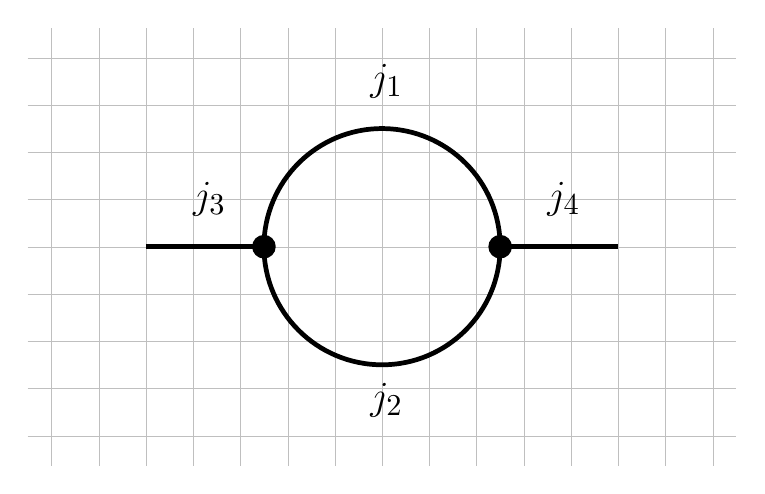
\begin{tikzpicture}[ thick,scale=3]
	
	% (VP_ml-B)
	\draw[gray!50,line width=0.01mm,step=0.2] (-0.5,0.073) grid (2.5, 1.927);
	\draw[line width=0.6mm] (1,1) circle (.5);
\fill (0.5,1) circle (0.05);
\fill (1.5,1) circle (0.05);
\draw[line width=0.6mm] (0, 1) -- (0.5, 1);
\draw[line width=0.6mm] (1.5, 1) -- (2, 1);
	\node at (1,1.7) {\fontsize{15pt}{0} $j_1$};
	\node at (1,0.35) {\fontsize{15pt}{0} $j_2$};
	\node at (0.25,1.2) {\fontsize{15pt}{0} $j_3$};
	\node at (1.75,1.2) {\fontsize{15pt}{0} $j_4$};


\end{tikzpicture}

\end{document}